\documentclass[a4paper,16pt]{article} 
\usepackage[left=1cm,right=1cm, 
 top=2cm,bottom=2cm,bindingoffset=0cm]{geometry} 
\usepackage[T2A]{fontenc} 
\usepackage{amsfonts} 
\usepackage{amsmath} 
\usepackage[utf8]{inputenc} 
\usepackage[english,russian]{babel} 

\usepackage{amsmath,amsfonts,amssymb,amsthm,mathtools,dsfont,physics,floatrow} 

\author{Никита Сухоруков, группа 825} 
\linespread{1.5} 
\title{Лабораторная работа 10.1\\
\textbf{Электронный парамагнитный резонанс}}
\date{}


\ifx\pdfoutput\undefined
\usepackage{graphicx}
\else
\usepackage[pdftex]{graphicx}
\fi



\begin{document}
\maketitle
\newpage
\section{Цель работы}
Исследовать электронный парамагнитный резонанс в молекуле дифенилпикрилгидразила $C_{18}H_{12}N_5O_6$ (ДФПГ), определить $g$-фактор электрона.
\begin{figure}[h!]
\centering	
\center{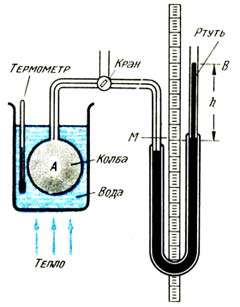
\includegraphics[scale=0.6]{2}}
\caption{Химическая структура молекулы ДФГП.}
\end{figure}
\section{Оборудование}

Параметры катушек:\\
Пробная катушка - $N$=49, $d$=(14.5$\pm$0.1) мм\\
Основная катушка - $N$=5500, $d$=(0.25$\pm$0.01) м\\
Модуляционная катушка - $N$=1500, $d$=(0.30$\pm$0.01) м\\
Погрешность вольтметра $GDM$-8145: $\pm0.03\%+4$ ед. младшего разряда\\
Погрешность частотометра $GFC-8010H$: $\pm5(10^{-6}+1\text{ ед. счета})$

\section{Измерения}

Находим резонансную частоту $f_0$ и частоту половинного сигнала $f_{\pm1/2}$
\begin{equation}
f_0=(125.3\pm0.1)\text{ МГц}, \hspace{10dd} f_{-1/2}=(124.6\pm0.1)\text{ МГц}, \hspace{10dd} f_{+1/2}=(125.9\pm0.1)\text{ МГц}
\end{equation}
Добротность
\begin{equation}
Q=\frac{f_0}{f_{+1/2}-f_{-1/2}}=96\pm15
\end{equation}
\begin{equation}
\Delta Q=\frac{1}{f_{+1/2}-f_{-1/2}}\Delta f_0+\frac{f_0}{(f_{+1/2}-f_{-1/2})^2}\Delta f_{-1/2}-\frac{f_0}{(f_{+1/2}-f_{-1/2})^2}\Delta f_{+1/2}=Q\left(\frac{\Delta f_0}{f_0}+\frac{\Delta f_{+1/2}+\Delta f_{-1/2}}{f_{+1/2}-f_{-1/2}}\right)
\end{equation}

Резонанс (ЭПР)\\
$U_R=(93.30\pm0.07)$ мВ - напряжение на $R$\\
$A_{\text{пол}}=(7.0\pm0.2)$ дел - размах резонансного пика в $X-Y$ развертке\\
$A_{1/2}=(1.6\pm0.1)$ дел - ширина на полувысоте\\
$E_i=(0.90\pm0.04)$ мВ - ЭДС на пробной катушке поднесенной к образцу\\
\begin{equation}
B_{\text{мод}}=\frac{2\sqrt{2}E_i}{\pi^2d^2N_{\text{проб}}\nu}=(0.50\pm0.03)\text{ мТл}, \hspace{5dd} \nu=50\text{ Гц}
\end{equation}
\begin{equation}
\varepsilon(B_{\text{мод}})=2\varepsilon(d)+\varepsilon(E_i)=\frac{2\cdot0.1}{14.5}+\frac{0.04}{0.90}=0.058
\end{equation}
\begin{equation}
\Delta B=\frac{A_{1/2}}{A_{\text{пол}}}B_{\text{мод}}=(0.11\pm0.02)\text{ мТл}
\end{equation}
\begin{equation}
\varepsilon(\Delta B)=\varepsilon(B_{\text{мод}})+\varepsilon(A_{1/2})+\varepsilon(A_{\text{пол}})=0.058+\frac{0.1}{1.6}+\frac{0.2}{7.0}=0.15
\end{equation}
\begin{figure}[h!]
\centering	
\center{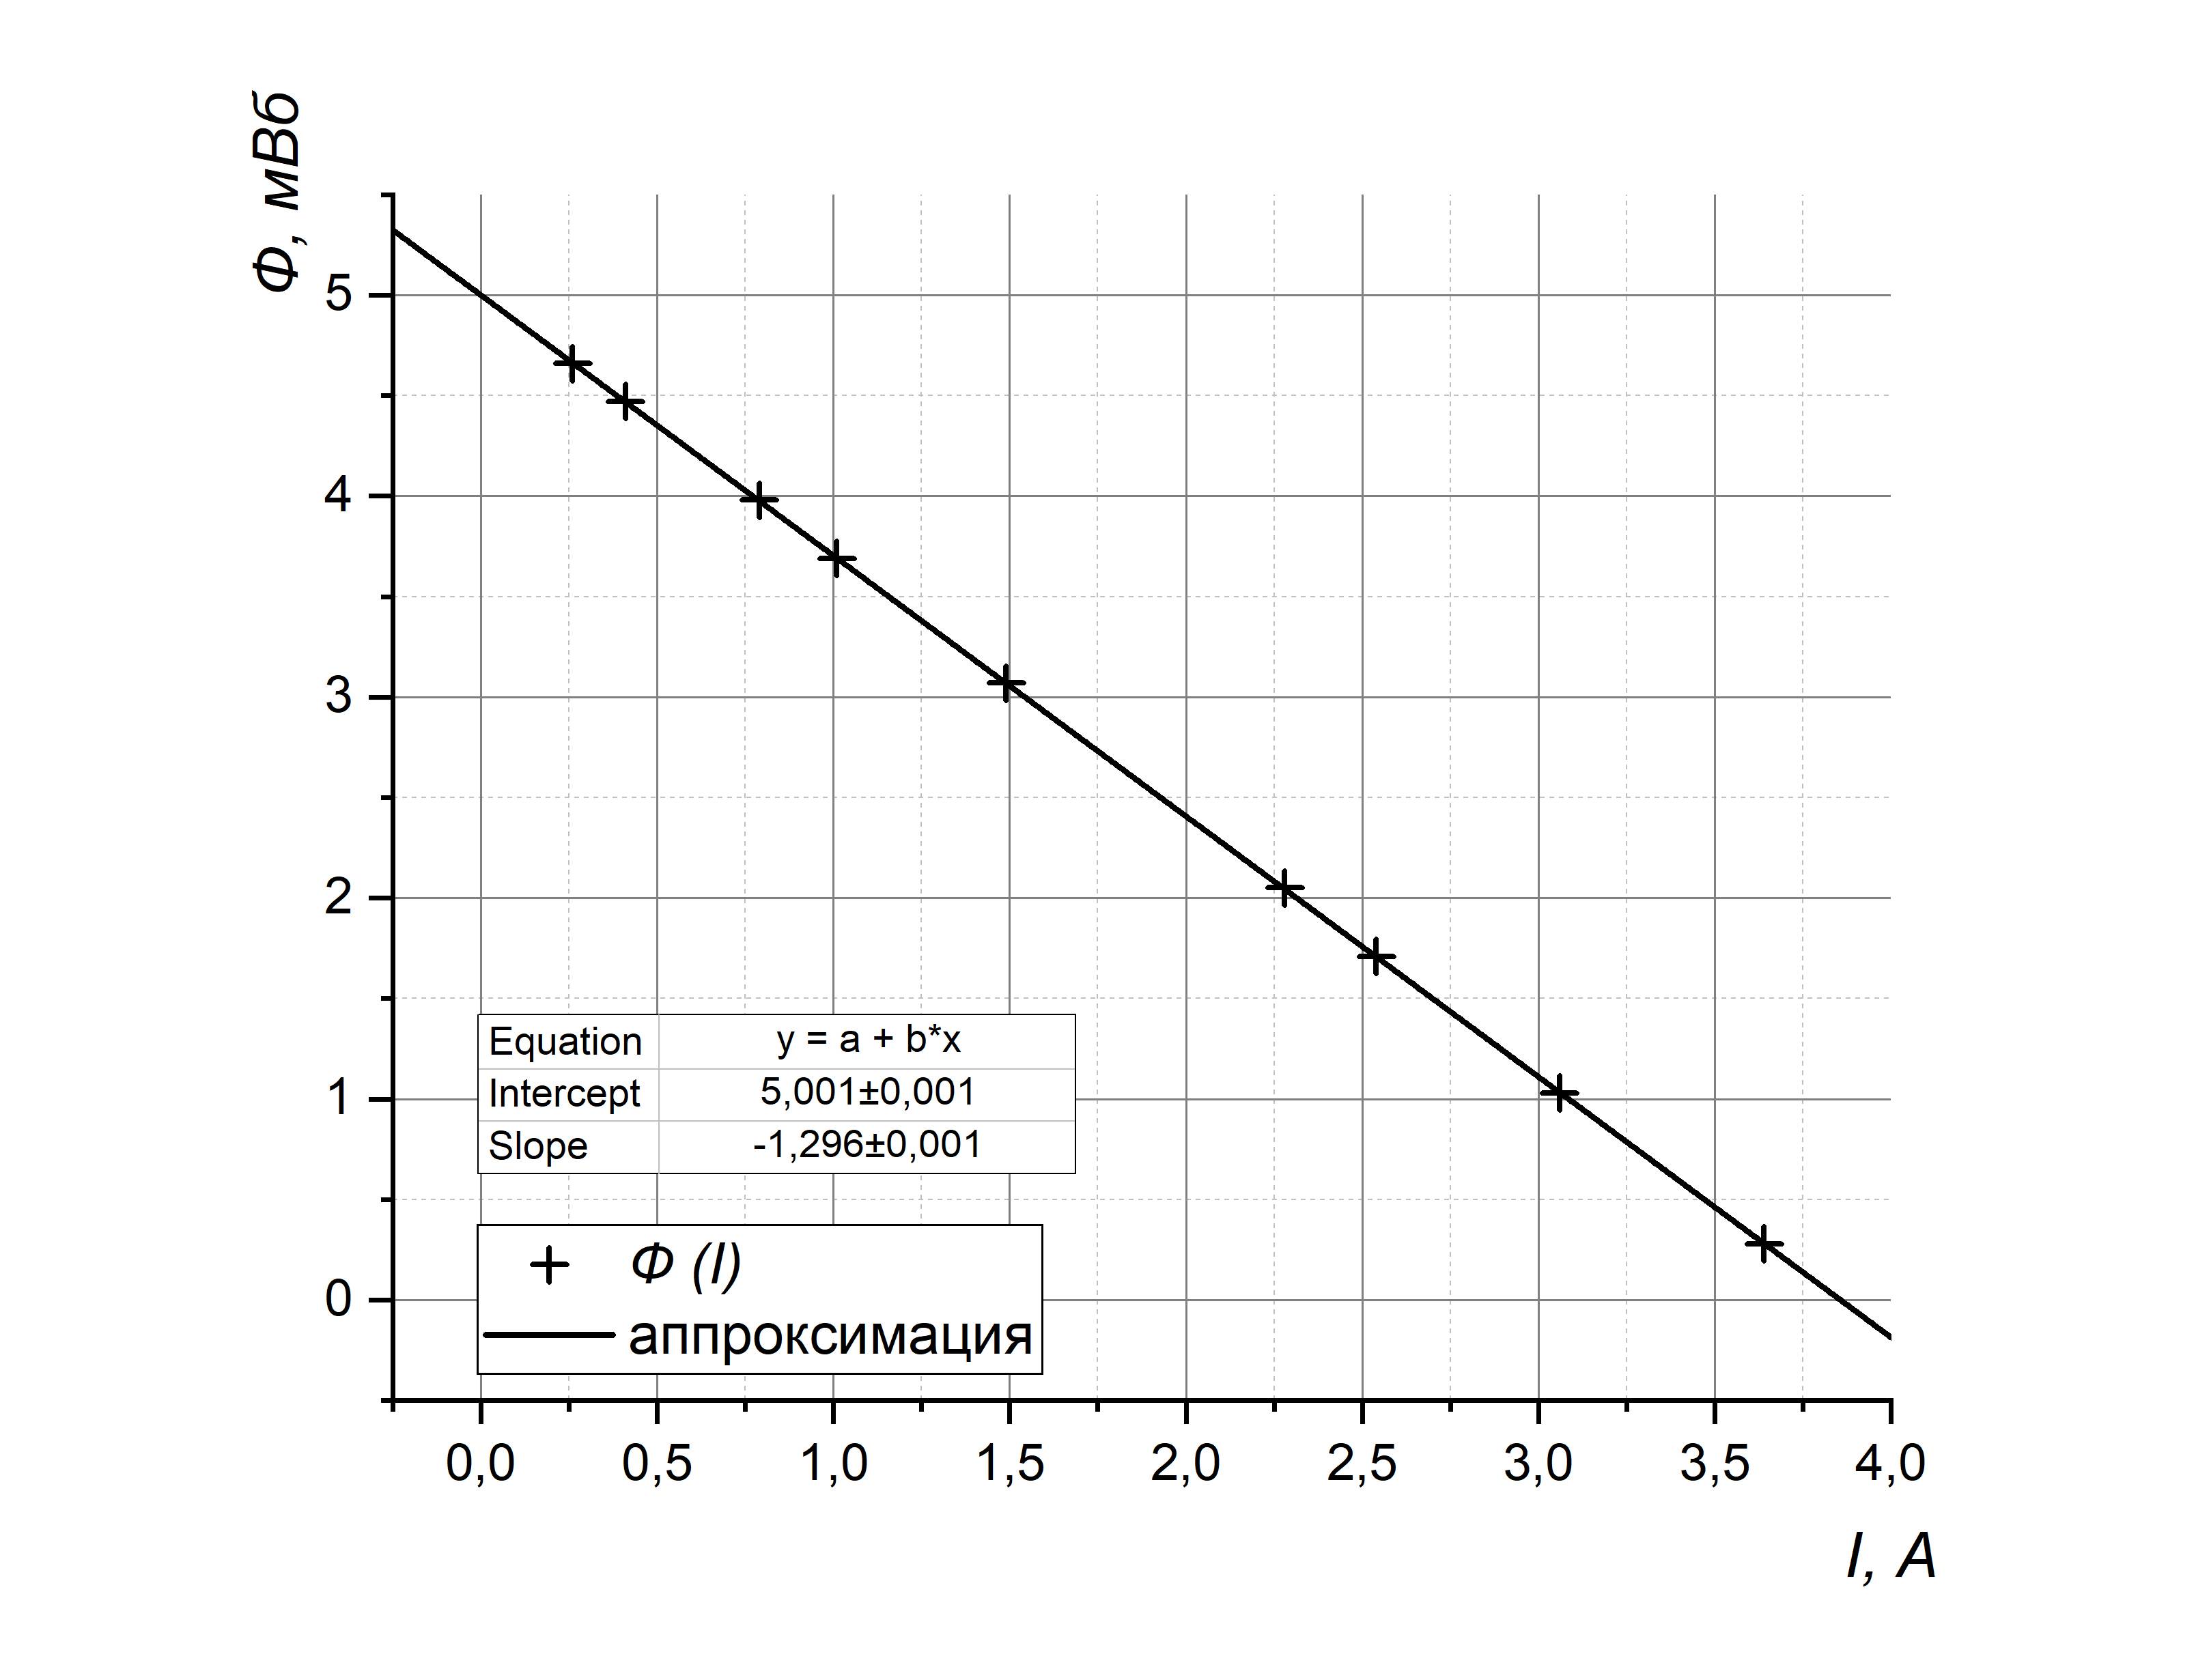
\includegraphics[scale=0.2]{4}}
\caption{Осциллограмма сигнала поглощения.}
\end{figure}

\begin{figure}[h!]
\centering	
\center{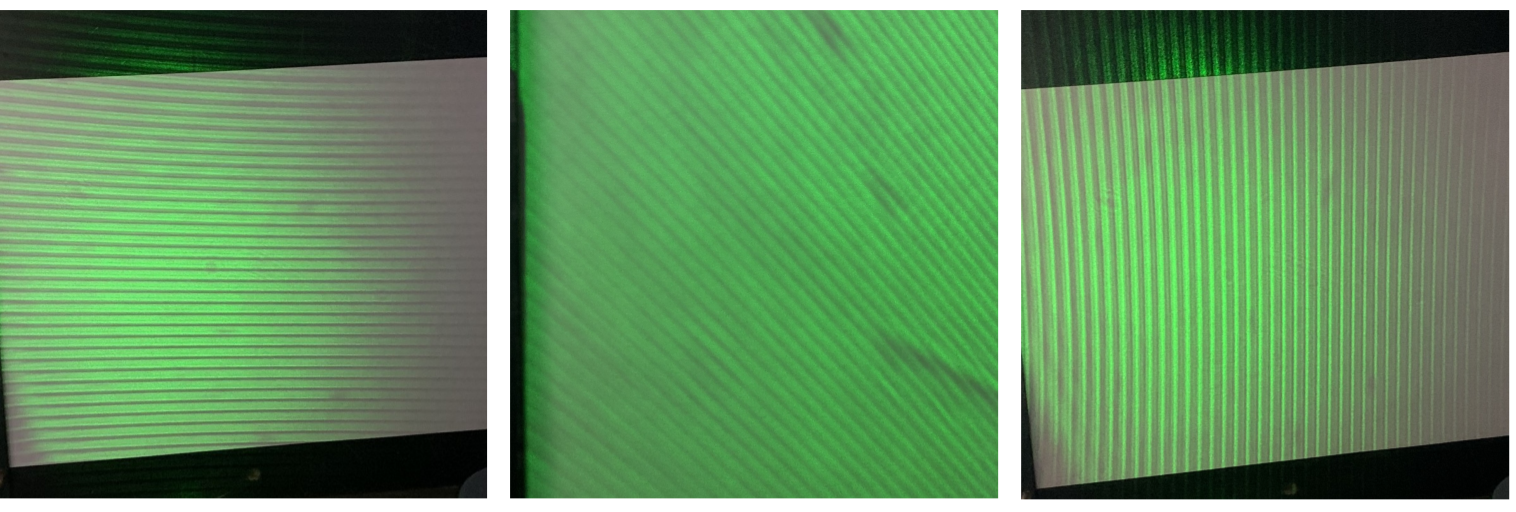
\includegraphics[scale=0.2]{3}}
\caption{Форма линии поглощения в режиме XY-развёртки при практически точной настройке.}
\end{figure}


\begin{center}
\begin{tabular}{| c | c | c | c | c | c |}
\hline
 $V_r, \text{ мВ}$ & $V_+, \text{ мВ}$ & $V_-, \text{ мВ}$ & $\Delta V_r, \text{ мВ}$ & $\Delta V_{+}, \text{ мВ}$ & $\Delta V_-, \text{ мВ}$\\ \hline
3.52 & 0.42 & 0.46 & 0.04 & 0.04 & 0.04 \\ \hline
5.35 & 0.61 & 0.69 & 0.04 & 0.04 & 0.04 \\ \hline
7.14 & 0.83 & 0.87 & 0.04 & 0.04 & 0.04 \\ \hline
8.90 & 1.06 & 1.08 & 0.04 & 0.04 & 0.04 \\ \hline
10.53 & 1.25 & 1.26 & 0.04 & 0.04 & 0.04 \\ \hline
\end{tabular}\\
\end{center}



\begin{figure}[h!]
\centering	
\center{\includegraphics[scale=0.8]{epr}}
\end{figure}
\begin{equation}
k_{min}^+=0.107, \hspace{5dd} k_{max}^+=0.130, \hspace{5dd} k_{min}^-=0.103, \hspace{5dd} k_{max}^-=0.126
\end{equation}
Из графика $k_{middle}=0.116\pm0.012$\\
Поле резонансного поглощения
\begin{equation}
B_0=\frac{4kU_R}{\pi\omega d^2N_{\text{проб}}}=(4.3\pm0.5)\text{ мТл}
\end{equation}
\begin{equation}
g=\frac{hf_0}{\mu_{\text{Б}}B_0}=(2.08\pm0.25)
\end{equation}
\begin{equation}
\varepsilon(B_0)=\varepsilon(k)+\varepsilon(U_R)+2\varepsilon(d)=0.12
\end{equation}
\begin{equation}
\varepsilon(g)=\varepsilon(f_0)+\varepsilon(B_0)=0.12
\end{equation}
\section{Вывод}

Табличное значение $g$-фактора $g_{theor}$=2.0036, что хорошо сходится с нашим значением $g_{exp}=(2.08\pm0.25)$. 
Резонанс возникал при $B_0=(4.3\pm0.5)$ мТл. Полуширина на полувысоте линии резонансного поглощения $\Delta B=(0.11\pm0.02)$ мТл.








\end{document}